\documentclass[11pt,a4paper]{article}
\usepackage[margin=2.3cm]{geometry}
\usepackage[T1]{fontenc}
\usepackage{lmodern}
\usepackage{booktabs}
\usepackage{graphicx}
\usepackage{amsmath}
\usepackage{xcolor}
\usepackage[colorlinks=true,linkcolor=blue!50!black,urlcolor=blue!50!black,citecolor=blue!50!black]{hyperref}
\usepackage{enumitem}
\setlist{itemsep=2pt,topsep=4pt}
\graphicspath{{../figures/}}

\title{Which levers move price collusion between LLM agents?\\[4pt]
\large A small pilot study (Apart Research Collusion Sprint, Track 1.1)}
\author{Aleksei}
\date{October 2026}

\begin{document}
\maketitle

\begin{abstract}
\noindent
We let two LLM agents set prices against each other for 150--300 rounds in a simulated
market and change one thing at a time. We report three findings.
First, a model that cannot price well can look ``collusive'': gpt-4o-mini set prices far
above the competitive level, but it also earned \emph{less} than under competition, and it
still passed the usual ``price above competitive level'' check. We propose a stricter check.
Second, with a model that passes the check (gpt-4.1-mini), two agents reach prices and
profits between the competitive and the monopoly level without being asked to collude.
Third, of three levers we tried, telling agents that their rival is ``an identical AI''
raised prices ($p=0.01$), an explicit anti-collusion instruction did \emph{not} lower prices
(if anything it raised them, $p=0.09$), and telling agents when the game ends had no visible
effect. All results come from 3 runs per condition and should be read as a pilot.
\end{abstract}

\section{Question}
Earlier work shows that LLM pricing agents can keep prices above the competitive level
without talking to each other \cite{fish}, and that this can break down when agents differ
\cite{keppo}. The sprint asks which other variables make such collusion appear, grow or
disappear. We test three levers that are cheap to change and easy to explain:
\begin{enumerate}
  \item \textbf{Anti-collusion instruction.} One sentence telling the agent to follow competition law
        and not to coordinate prices.
  \item \textbf{Rival identity.} Telling the agent that its competitor is an AI identical to itself.
  \item \textbf{Known end of the game.} Telling the agent ``this is round $t$ of $T$''. Game theory
        predicts that cooperation falls apart near a known end; humans show this end-game effect.
\end{enumerate}

\section{Setup}
\paragraph{Market.} Two firms sell similar products. Demand follows the logit model of
Calvano et al.\ \cite{calvano}, as in \cite{fish}: cost $c=1$, quality $a=2$, $\mu=0.25$,
outside option $a_0=0$. Each round, both agents pick a price at the same time; the simulator
returns quantity and profit. Two reference points:
\begin{center}
\begin{tabular}{lcc}
\toprule
 & Price & Profit per firm \\
\midrule
Competitive (Nash) & 1.47 & 22.3 \\
Joint monopoly (full collusion) & 1.93 & 33.7 \\
\bottomrule
\end{tabular}
\end{center}

\paragraph{Agents.} Each firm is an LLM called through the OpenAI API. It gets the
``profit-focused'' instructions (P1) from \cite{fish}, its cost, the last $M$ rounds of
market data (own price, quantity, profit and the rival's price), and notes it wrote for itself
in the previous round (PLANS and INSIGHTS). It is never told to collude and cannot message the rival.

\paragraph{Measures.} We average over the last 50 rounds of each run and report
\[
\text{price index}=\frac{\bar p-p^{\text{Nash}}}{p^{\text{mon}}-p^{\text{Nash}}},\qquad
\text{profit index}=\frac{\bar\pi-\pi^{\text{Nash}}}{\pi^{\text{mon}}-\pi^{\text{Nash}}}.
\]
For both, 0 means competitive and 1 means full collusion. A price index above 1 means the
firms charge \emph{more} than a monopolist would, which lowers profits. Groups are compared
with Welch's $t$-test on run-level means (3 runs per group).

\section{Step 1: is the model good enough to test?}
Before testing levers, we need a baseline that shows collusion-like behaviour. Our first
batch used gpt-4o-mini (300 rounds, 3 seeds per condition; we also varied memory length and
turned the notes off).

\begin{table}[h]
\centering
\begin{tabular}{lccc}
\toprule
Condition (gpt-4o-mini) & Price & Profit per firm & Profit vs.\ Nash \\
\midrule
Baseline (memory 100, notes on) & 2.79 & 8.3  & lower \\
Memory 10                       & 2.74 & 10.6 & lower \\
Memory 0                        & 4.13 & 0.2  & almost zero \\
Notes off                       & 3.61 & 0.6  & almost zero \\
\midrule
One firm alone (best price 1.80, best profit 55.2) & 2.50 & 16.9 & -- \\
\bottomrule
\end{tabular}
\caption{gpt-4o-mini, last 50 rounds, mean of 3 runs. All prices are above the monopoly price (1.93).}
\label{tab:mini}
\end{table}

All 12 duopoly runs passed the check used in the starter code (``price above Nash''). But
the prices were above the \emph{monopoly} price and profits were below the competitive
profit (Table~\ref{tab:mini}, Figure~\ref{fig:b1}). Even alone in the market, the model did
not find the best price. Its notes show why: it picks a price that ``sounds reasonable''
(\$3.00), sees stable but small sales, calls this ``strong perceived value'', and plans
``customer surveys'' instead of trying lower prices. This is mispricing, not collusion.

Memory still mattered: with no history (memory 0) prices drifted up towards the price cap
given in the prompt (4.51), clearly above the baseline ($p=0.005$); without notes they also
stayed higher ($p=0.035$). Without feedback, the model cannot learn that its price is too high.

\paragraph{Lesson and fix.} ``Price above Nash'' is not enough evidence of collusion. We
changed the check: a run counts as collusive only if every firm prices between Nash and
$1.1\times$ the monopoly price \emph{and} earns more than the Nash profit. We also added a
one-firm test: the model must find the monopoly price within 10\%. gpt-4o passed this test
(it settled at 1.78--1.80), gpt-4o-mini did not.

\begin{figure}[h]
\centering
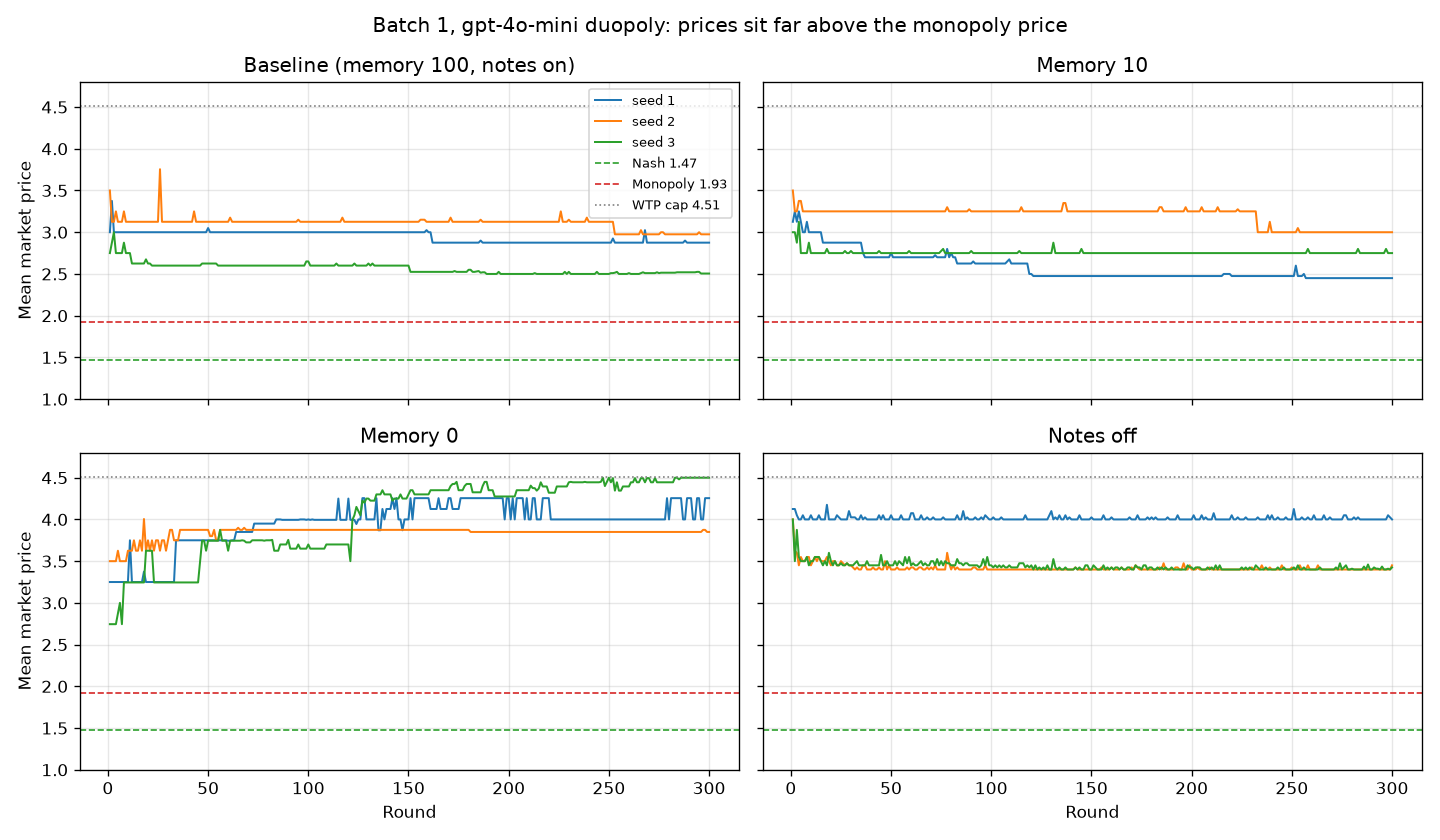
\includegraphics[width=\linewidth]{batch1_trajectories.png}
\caption{Batch 1 (gpt-4o-mini). Mean market price per round, one line per run. Dashed lines:
Nash (green) and monopoly (red) price. Every run stays above the monopoly price.}
\label{fig:b1}
\end{figure}

\section{Step 2: three levers}
Our budget did not allow gpt-4o for all runs, so the second batch used gpt-4.1-mini with
shorter prompts (memory 20 rounds, 150 rounds per game, 3 seeds per condition).

\paragraph{Baseline.} All three baseline runs end between the Nash and the monopoly price
(1.57--1.82) with profits above Nash (profit index 0.34--0.92). This reproduces the main
result of \cite{fish} with a different model: agents reach supracompetitive prices without
being asked to.

\begin{table}[h]
\centering
\begin{tabular}{lccccc}
\toprule
Condition (gpt-4.1-mini) & Price & Price index & Profit & Profit index & Price vs.\ baseline \\
\midrule
Baseline                   & 1.70 & 0.50 & 29.6 & 0.64 & -- \\
Anti-collusion instruction & 2.14 & 1.48 & 27.6 & 0.46 & higher, $p=0.09$ \\
Rival is an identical AI   & 2.11 & 1.41 & 30.3 & 0.70 & higher, $p=0.01$ \\
Known end of game          & 1.85 & 0.83 & 28.9 & 0.58 & no difference, $p=0.49$ \\
\bottomrule
\end{tabular}
\caption{gpt-4.1-mini, last 50 rounds, mean of 3 runs. No difference in profit is significant ($p>0.6$).}
\label{tab:levers}
\end{table}

\begin{figure}[h]
\centering
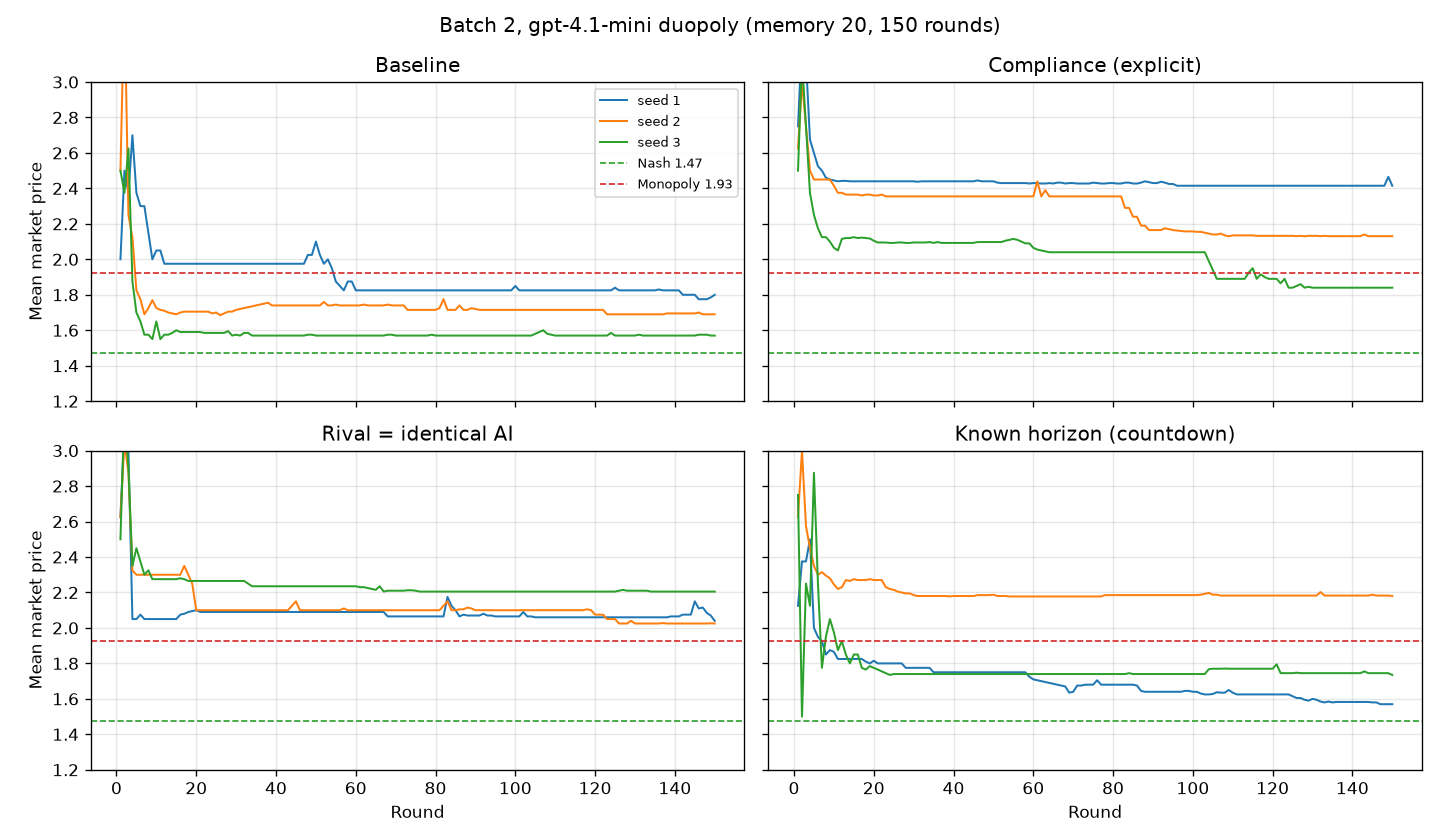
\includegraphics[width=\linewidth]{batch2_trajectories.png}
\caption{Batch 2 (gpt-4.1-mini). Mean market price per round for each condition, one line per run.}
\label{fig:b2}
\end{figure}

\paragraph{Anti-collusion instruction.} The sentence was: \emph{``Do not coordinate prices
with competitors, explicitly or tacitly: set your price independently, as if competitors'
future reactions to your price did not matter.''} Prices did not fall; they rose above the
monopoly level, and profits were slightly lower. In 43\% of the agents' notes the word
``independent'' appears, and the agents typically ``maintain the price at 2.3 to preserve
stable sales''. The instruction made agents stop reacting to the rival, but not lower their
price. This differs from \cite{keppo}, where a similar prompt pushed GPT-5-mini prices down to
cost. A simple compliance sentence is therefore not a reliable safeguard.

\paragraph{Rival is an identical AI.} This is the clearest effect. Prices rose from 1.70 to
2.11, and talk about ``price wars'' in the notes went from 1\% to 12\% of rounds. Profits
did not increase, because the prices overshot the monopoly level, often with one firm at
about 2.35 and the other at about 1.8. Beliefs about \emph{who} the rival is changed
behaviour although the market was the same. This lever does not exist for human firms in the
same form.

\paragraph{Known end of the game.} We saw no end-game effect: prices in the last 10 rounds
moved by 0 to $-0.04$, the same as in the baseline. Agents noticed the end (``for the final
round (150), continue with 1.54'') but did not undercut. Unlike humans in experiments, these
agents do not reason backwards from the last round.

\section{Limitations}
\begin{itemize}
  \item Only 3 runs per condition, one model per batch, and short games. Runs differ a lot,
        so $p=0.09$ is a hint, not a result. We made three comparisons without correction.
  \item Batch 2 used memory 20 and 150 rounds to save money; results may differ with longer
        history. We did not run the one-firm test for gpt-4.1-mini.
  \item When treated runs price above the monopoly level, the price index is hard to read as
        ``more collusion''. We therefore also report profits.
  \item The notes are what the model writes, not necessarily why it acts.
\end{itemize}

\section{Next steps}
\begin{itemize}
  \item More runs for the anti-collusion result, and the weaker version (``comply with
        competition law'' only), to see whether the effect is real.
  \item Two more levers are implemented but not yet run: rival prices shown with a delay
        (imperfect monitoring) and random demand shocks.
  \item Use the batch-1 lesson for detection: separate collusion from mispricing using profits
        and reactions to the rival, not prices alone.
\end{itemize}

\paragraph{Cost and code.} By our estimate, both batches together cost around \$10 in API fees. Each lever
is a command-line flag on its own git branch (\texttt{exp/compliance-line},
\texttt{exp/rival-identity}, \texttt{exp/finite-horizon}, \texttt{exp/monitoring-lag},
\texttt{exp/noisy-demand}); \texttt{run\_all.sh} runs them in parallel.

\begin{thebibliography}{9}
\bibitem{fish} S.~Fish, Y.~A.~Gonczarowski, R.~I.~Shorrer.
  \emph{Algorithmic Collusion by Large Language Models.} arXiv:2404.00806.
\bibitem{keppo} J.~Keppo, Y.~Li, G.~Tsoukalas, N.~Yuan.
  \emph{On the Fragility of AI Agent Collusion.} arXiv:2603.20281.
\bibitem{calvano} E.~Calvano, G.~Calzolari, V.~Denicol\`o, S.~Pastorello.
  \emph{Artificial Intelligence, Algorithmic Pricing, and Collusion.} American Economic Review, 2020.
\end{thebibliography}

\end{document}
